\section{Introduction}

As a free online service, VirusTotal~\cite{virustotal} analyzes files submitted by real-world users to identify many different kinds of malwares, 
like viruses, worms, trojans, and so on. 
VirusTotal applies different antivirus engines to each submitted file and generate an aggregated reports. 
All submitted files and generated reports are saved and can be accessed through public API. 


The repository on VirusTotal provides a good source to conduct data mining. 
There are huge amount of data on VirusTotal.
Figure~\ref{fig:subnum} shows the number of distinct files submitted from 05/08/2016 to 05/14/2016. 
We can see that there are more than 10 million distinct suspicious files submitted each day. 
This amount of data makes VirusTotal a rough estimation of malwares in the real world. 
All data on VirusTotal are labeled by state-of-the-art antivirus techniques. 
VirusTotal update each antivirus engine every 5 minutes. 
Besides whether a given a submitted file is detected by an antivirus engine, VirusTotal also keeps exact detection tag returned by each engine. 
There are also online active malware researchers, 
who comment and vote each submitted file and serve as an important supplement of antivirus engines. 
We believe mining data on VirusTotal would enable many ``Big Security'' applications. 

In industry, antivirus vendors widely use VirusTotal data to reduce false negatives and false positives from their products. 
{\bf [TODO. Discuss how academic people use VirusTotal, and use Heqing’s work as an example]} 

In this paper, we view data on VirusTotal as a stream, based on each submitted file’s ``first seen'' time, 
and design two stream mining applications: hot malware family mining and malware prediction. 
There are possible infinite possible malware families. 
Hot malware family mining can precisely identify malware families, 
which occupy more than a given percentage of total malwares, by using a constant number of counters.  
We think malwares in different family does not appear uniformly across time, and they appear in bursts. 
We built a cache-based algorithm to predict malwares in which family would appear in the near future. 

In summary, we made the following contributions in this paper:

\begin{figure}[t!]
\begin{center}
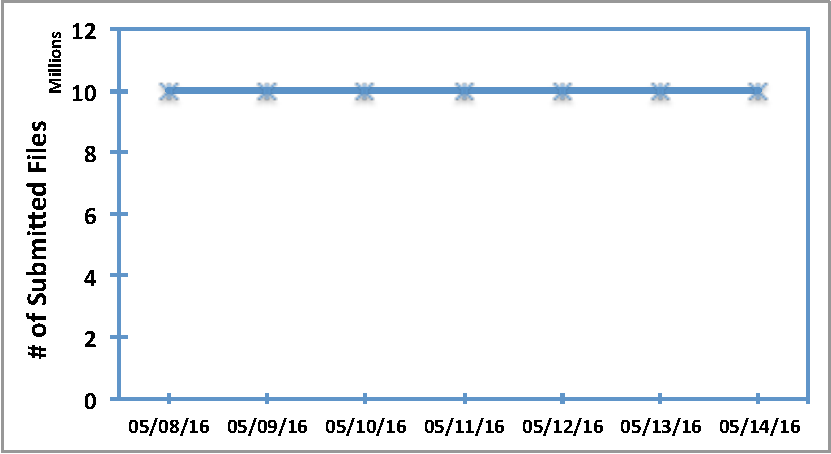
\includegraphics[width=2.5in]{figure/submission_number}
\caption{The number of files submitted to VirusTotal from 05/08/2016 to 05/14/2016. 
{\bf [TODO: All numbers in this figure are made up, and they must be changed later.]}}
\label{fig:subnum}
\end{center}
\end{figure}
